Considering the context of our study, understanding the running components (operating systems, file systems, services) in the router's firmware contributes to the re-hosting.  Re-hosting is a technique for executing a tightly coupled system in another hardware or platform (in our case, it means emulating the router firmware in a general-purpose computer desktop).  Thus, our contribution relies upon this context.  We observed different approaches regarding overcoming re-hosting difficulties caused by the need for peripherals of the original hardware that are not present in the emulated device (the most challenging aspect of emulating a firmware). For example, the work of \cite{firmware-challenges} surveys the prominent techniques used in firmware re-hosting to bypass actual hardware dependency. Thereby, the four most common approaches are Partial Emulation, Fuzzing, Learning, and Abstraction Replacement. Also, a recent article discusses a novel approach that we will call here Symbolic Inference. We will briefly describe these approaches in the following sections.

\section{Partial Emulation}

Partial emulation, also known as ``hardware in the loop'', consists of emulating most firmware execution; however, redirecting to the actual device hardware calls when the firmware asks for a peripheral is infeasible. This approach requires having an actual device available, and for this reason, it does not scale. Execution fidelity, on the other hand, is pretty close to the actual hardware execution. The work of \cite{surrogates} enhances hardware redirecting by building a hardware bridge using an FPGA board to connect the PCI bus on the emulating host with the PCI bus on the actual embedded device, an approach they called {\tt SURROGATES}. Figure \ref{fig:surrogates} illustrates the approach used for the {\tt SURROGATES} solution.

\begin{figure}[H]
    \centering
    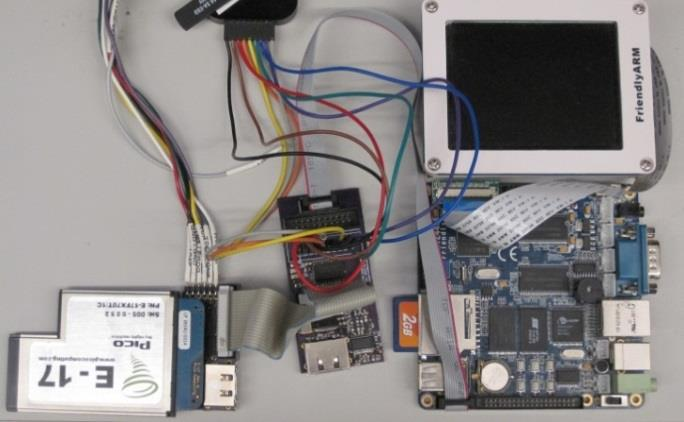
\includegraphics[width=0.7\textwidth]{figs/surrogates.png}
    \caption{FPGA gateway built to forward peripheral calls from the emulated system to the real device hardware. Developed as part of {\tt SURROGATES} solution \cite{surrogates}.}
    \label{fig:surrogates}
\end{figure}
The work of \cite{avatar2} extensively explores vulnerability discovery in embedded devices using the hardware in the loop technique. They use a symbolic engine builds upon QEMU called {\tt S2E} to search for vulnerabilities in IoT devices through re-hosting and to redirect peripherals calls to the actual hardware. In addition, they implement a tool called {\tt Avatar$^2$} as a reverse engineering framework based on the hardware in the loop approach.  Nonetheless, the dependency on the physical systems imposes barriers in testing and makes this alternative infeasible for our research.

\section{Fuzzing}

To overcome the partial emulating techniques, Fuzzing is a re-hosting approach to hardware dependence (not to be confused with fuzzing as a vulnerability discovery technique) because hardware calls to peripherals do not need the peripheral to be successful. Instead, the actual peripheral response request to the hardware call is just a binary value. Therefore, knowing the range of values that provide an acceptable answer to the hardware call, selecting any random value within this range is enough to keep executing the emulated system.

\cite{p2im} effectively implements this kind of hardware bypass.  The authors present an approach to model the interface between the processor and the peripheral. The method suggested is called {\tt P2IM} - Processor-Peripheral Interface Modeling.  However, it requires a human specialist to model the interface between the CPU and a specific peripheral to determine the specific range of values to each hardware call. Therefore, this approach also does not provide a scalable solution, requiring human intervention (to model the interface).

\section{Learning}

Learning is a similar approach to fuzzing for re-hosting, as it relies on the fact that to bypass hardware dependence, it is only needed to return expected values to hardware calls. However, the learning approach, as used in \cite{pretender} first monitors actual hardware execution and registers each hardware-peripheral interaction. Then it uses a Machine Learning algorithm to build a model of the interface (in contrast to using a human specialist as in the fuzzing approach). As a result, the learning technique produces a better interface to simulate peripheral interaction; however, it also depends on having the actual hardware first to build the interface's working model, which impedes its scalability and makes it an unsuitable solution for us.

\section{Abstraction Replacement}

Abstraction Replacement takes a different approach, and instead of producing answers to hardware calls that are similar to the responses real hardware would produce, this method tries to remove from the original firmware the hardware call, replacing it with another abstraction not requiring the actual hardware.

In the work of \cite{halucinator}, they develop the method called {\tt HALucinator}, whose idea is to search for Hardware Abstraction Layer (HAL) libraries inside the firmware and replace those libraries with custom libraries implemented by the researchers that do not require peripherals to work. However, this method still requires human intervention for each firmware and thus, still does not scale.

On the other hand, the work of \cite{firmadyne} implements a tool called {\tt Firmadyne}, whose approach to re-hosting consists of replacing the original kernel found on the firmware image with a custom implemented and instrumented kernel worked by their team (the same kernel is used to all firmware images emulated, regardless of their original kernel version) together with applying some fixes to the filesystem (e.g replacing default root password and creating some essential directories). This approach allows firmware emulation to be done at scale, with the counterpart that the kernel replacement sacrifices emulation fidelity (because of the change in the kernel, emulation fidelity in userspace at most). The authors of {\tt Firmadyne} also implemented a web scraper capable of downloading firmware binary from popular vendors websites and then used {\tt Firmadyne} to emulate and perform security analysis on the downloaded firmware images.

Firmadyne architecture, shown in Figure \ref{fig:firmadyne}, is very much aligned with the architecture we first idealized for our research, and thus this tool will set the basis of the work presented in this paper. More details about Firmadyne architecture will be given in Chapter \ref{chap:screen}.

\begin{figure}[H]
    \centering
    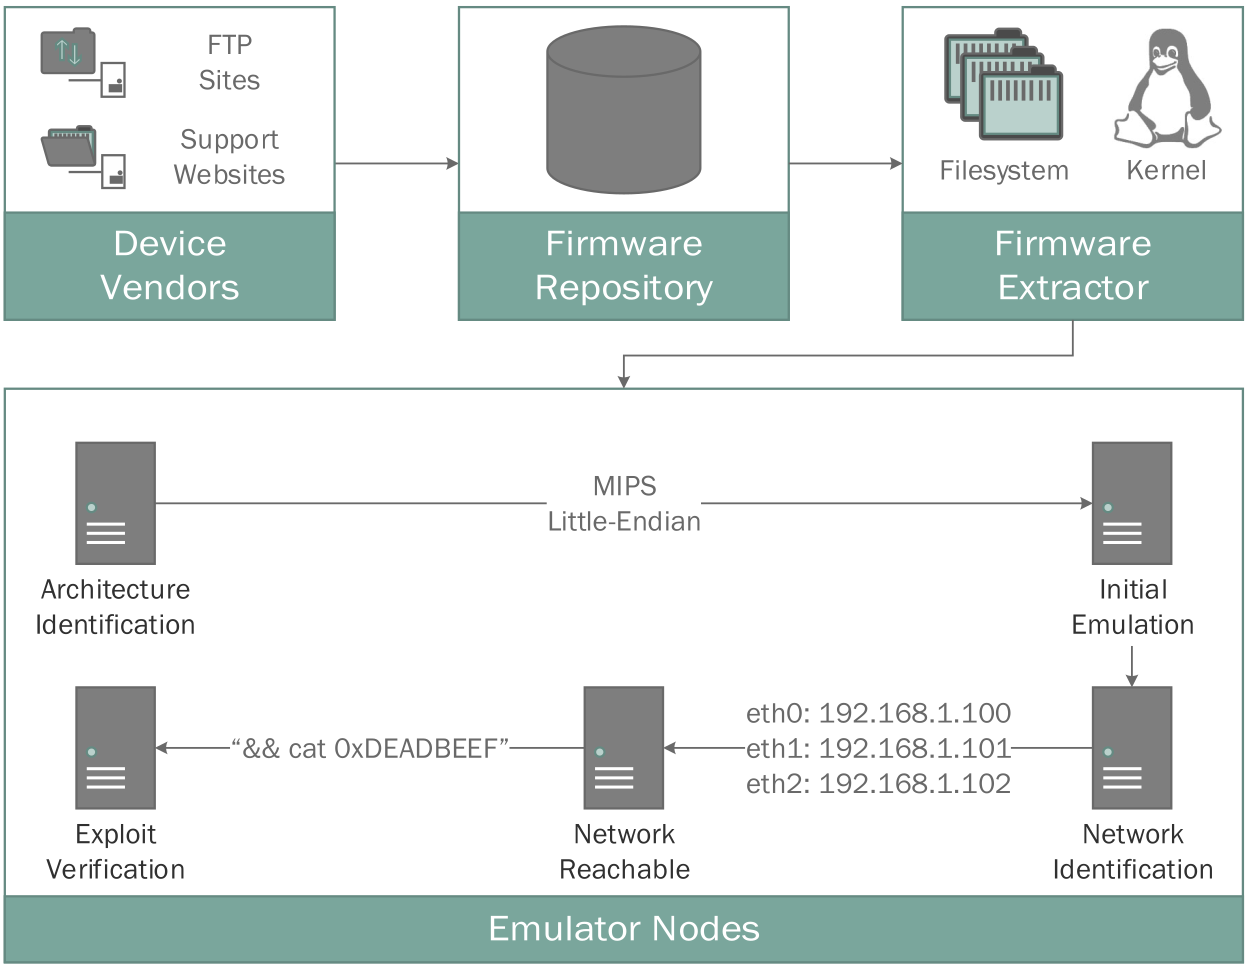
\includegraphics[width=0.6\textwidth]{figs/firmadyne.png}
    \caption{Firmadyne architecture~\cite{firmadyne}.}
    \label{fig:firmadyne}
\end{figure}

\section{Symbolic Inference}

A new approach to firmware emulation was proposed in the work of \cite{jetset}, in which the researchers hypothesize that the minimal behavior expected to boot firmware to a point of interest by a security analyst could be inferred automatically. They then implemented a tool called Jetset that extends the idea of symbolic execution to model the hardware peripherals calls answers until firmware reaches a target address (e.g. boot finished). Their solution takes as inputs the executable code of the target, the memory layout of the target, the entry point address for execution start, and the goal address that the analyst desires the code to reach.

The authors of Jetset then prove the capacities of their implemented tool by using it to perform the re-hosting of thirteen different pieces of firmware. The device in which Jetset was applied that resembles the most similarities with wireless routers is the Raspberry Pi 2 (based on the Broadcom BCM2836 System on a Chip [SoC] running on ARM architecture). For this device, the inputs needed for the proposed method to succeed are pieces of information extracted from the chip manufacturer documentation for the chip (datasheet). In terms of scalability, this is not ideal because one needs to gather information about the different SoC's of our targets, but the idea behind Jetset is very powerful and is a solution worth exploring.

\section{Summary}

% As we can see, many of the re-hosting techniques rely on non-scalable mechanisms. For example, Firmadyne provides an improvement to enable analysis at scale; however, it imposes limitations and remove much software running in kernel mode.  We present a proposal that differs from others by increasing the re-hosting coverage of operating systems in small and home-office systems (SOHO).  Our work provides a vision of operating systems to focus on, including a hardware architecture, version, and file systems.  Hence, identify dependencies in components (specific drivers) and maximize artifacts with favorable prominence (e.g., network stack).  As a result, it advances the state-of-the-art by bringing pieces of software left out of the emulation loop.

% ======== AQUI TEM MUDANÇA IMPORTANTE ========
As we can see, many of the re-hosting techniques rely on non-scalable mechanisms. For example, Firmadyne provides an improvement to enable analysis at scale; however, it imposes limitations and removes much software running in kernel mode. As in our work we are targeting a specific class of firmware, in this case, wireless routers running on SOHO systems, we propose to make an adjustment in the approaches used for firmware re-hosting to use information gathered from freely available firmware images on the internet and use these pieces of information to enumerate firmware images features and components. This enumeration can be used to highlight prominent targets for security inspection and also to enhance the approach used for re-hosting. For instance, the kernel replacement done by Firmadyne could be done with a kernel more similar to the original kernel found on the firmware. 

In the next section, we will further discuss the approach that is going to be used in our research.